% Template KLTN cho SV trường ĐHKHTN
% Liên hệ: bhthong@fit.hcmus.edu.vn
% Last update: 

% Chú ý: đọc các phần chú ý đóng khung của file này và chỉnh lại cho phù hợp.
% Trước khi build, xóa hết các file được tạo ra trong quá trình build trước đó, và build theo thứ tự: BIB > PDF > PDF.
% Nếu cập nhật tài liệu tham khảo, cũng cần build lại theo cách trên.

\documentclass[oneside,a4paper,14pt]{extreport}

% Font tiếng Việt
\usepackage[T5]{fontenc}
\usepackage[utf8]{inputenc}
\DeclareTextSymbolDefault{\DH}{T1}

% Tài liệu tham khảo
\usepackage[
	sorting=nty,]{biblatex}
\usepackage[unicode]{hyperref} % Bookmark tiếng Việt
\addbibresource{References/references.bib}

\makeatletter
\def\blx@maxline{77}
\makeatother

% Chèn hình, các hình trong luận văn được để trong thư mục Images/
\usepackage{graphicx}
\graphicspath{ {Images/} }

% Chèn và định dạng mã nguồn
\usepackage{listings}
\usepackage{color}
\definecolor{codegreen}{rgb}{0,0.6,0}
\definecolor{codegray}{rgb}{0.5,0.5,0.5}
\definecolor{codepurple}{rgb}{0.58,0,0.82}
\definecolor{backcolour}{rgb}{0.95,0.95,0.92}
\lstdefinestyle{mystyle}{
    backgroundcolor=\color{backcolour},   
    commentstyle=\color{codegreen},
    keywordstyle=\color{magenta},
    numberstyle=\tiny\color{codegray},
    stringstyle=\color{codepurple},
    basicstyle=\footnotesize,
    breakatwhitespace=false,         
    breaklines=true,                 
    captionpos=b,                    
    keepspaces=true,                 
    numbers=left,                    
    numbersep=5pt,                  
    showspaces=false,                
    showstringspaces=false,
    showtabs=false,                  
    tabsize=2
}
\lstset{style=mystyle}

% Chèn và định dạng mã giả
\usepackage{amsmath}
\usepackage{algorithm}
\usepackage[noend]{algpseudocode}
\makeatletter
\def\BState{\State\hskip-\ALG@thistlm}
\makeatother

% Bảng biểu
\usepackage{multirow}
\usepackage{array}
\newcolumntype{L}[1]{>{\raggedright\let\newline\\\arraybackslash\hspace{0pt}}m{#1}}
\newcolumntype{C}[1]{>{\centering\let\newline\\\arraybackslash\hspace{0pt}}m{#1}}
\newcolumntype{R}[1]{>{\raggedleft\let\newline\\\arraybackslash\hspace{0pt}}m{#1}}

% Đổi tên mặc định
% \renewcommand{\chaptername}{Chapter}
% \renewcommand{\figurename}{Figure}
% \renewcommand{\tablename}{Table}
% \renewcommand{\contentsname}{Table of contents}
% \renewcommand{\listfigurename}{List of figures}
% \renewcommand{\listtablename}{List of tables}
% \renewcommand{\appendixname}{Appendix}

% Kích thước Chapter
\usepackage{titlesec}
\titleformat{\chapter}[display]
  {\LARGE\bfseries}
  {\chaptertitlename\ \thechapter}{18pt}{\huge}


% Dãn dòng 1.5
\usepackage{setspace}
\onehalfspacing

% Reference: https://tex.stackexchange.com/questions/171999/overfull-hbox-in-biblatex
\emergencystretch=1em

% Thụt vào đầu dòng
\usepackage{indentfirst}

% Canh lề
\usepackage[
  top=30mm,
  bottom=25mm,
  left=30mm,
  right=20mm,
  includefoot]{geometry}
  
% Trang bìa
\usepackage{tikz}
\usetikzlibrary{calc}
\newcommand\HRule{\rule{\textwidth}{1pt}}

% Section depth
\newcommand{\subsubsubsection}[1]{\paragraph{#1}\mbox{}\\}
\setcounter{secnumdepth}{4}
\setcounter{tocdepth}{4}
% common math syntax
\usepackage{commath}
% For attaching proposal
\usepackage{pdfpages}
\usepackage{amssymb}
% ========================================================================================= %
% CHÚ Ý: Thông tin chung về KLTN - sinh viên điền vào đây để tự động update các trang khác  %
% ========================================================================================= %
\newcommand{\tenSV}{Mai~Duy~Nam~-~Nguyễn~Hữu~Bình} % Dấu ~ là khoảng trắng không được tách (các chữ nối với nhau bằng dấu ~ sẽ nằm cùng 1 dòng
\newcommand{\mssv}{1234567}
\newcommand{\tenKL}{Sử~dụng~LaTeX trong Khoá~luận~tốt~nghiệp} % Chú ý dấu ~ trong tên khóa luận
\newcommand{\tenGVHD}{Tên~Giáo~Viên}
\newcommand{\tenBM}{Công nghệ tri thức}

\newcommand\numExperimentedMethods{eight}

\begin{document}

\begin{titlepage}

\begin{center}
%ĐẠI HỌC QUỐC GIA THÀNH PHỐ HỒ CHÍ MINH\\
UNIVERSITY OF SCIENCE\\
\textbf{FACULTY OF INFORMATION TECHNOLOGY}\\[2cm]


{ \Large \bfseries Mai Duy Nam - Nguyễn Hữu Bình\\[2cm] } 

%Tên đề tài Khóa luận tốt nghiệp/Đồ án tốt nghiệp

{ \Large \bfseries THE DISAGREEMENT PROBLEM IN XAI ON IMAGE DATA VIA SALIENCY MAPS\\[3cm]} 


%Chọn trong các dòng sau
\large BACHELOR THESIS\\
%\large ĐỒ ÁN TỐT NGHIỆP CỬ NHÂN\\
%\large THỰC TẬP TỐT NGHIỆP CỬ NHÂN\\
%Đưa vào dòng này nếu thuộc chương trình Chất lượng cao, hoặc lớp Cử nhân tài năng
\large HONORS PROGRAM\\
%\large CHƯƠNG TRÌNH CHẤT LƯỢNG CAO\\
%\large CHƯƠNG TRÌNH CỬ NHÂN TÀI NĂNG\\[2cm]


\begin{tikzpicture}[remember picture, overlay]
  \draw[line width = 2pt] ($(current page.north west) + (2cm,-2cm)$) rectangle ($(current page.south east) + (-1.5cm,2cm)$);
\end{tikzpicture}

\vfill
Ho Chi Minh City, June 2022

\end{center}

\pagebreak



\begin{center}

UNIVERSITY OF SCIENCE\\
\textbf{FACULTY OF INFORMATION TECHNOLOGY}\\[2cm]


{\large \bfseries Mai Duy Nam - 19120298\\} 
{\large \bfseries Nguyễn Hữu Bình - 19120460\\[2cm]}

%Tên đề tài Khóa luận tốt nghiệp/Đồ án tốt nghiệp

{ \Large \bfseries THE DISAGREEMENT PROBLEM IN XAI ON IMAGE DATA VIA SALIENCY MAPS\\[2cm] } 


%Chọn trong các dòng sau
\large BACHELOR THESIS\\
%\large ĐỒ ÁN TỐT NGHIỆP CỬ NHÂN\\
%Đưa vào dòng này nếu thuộc chương trình Chất lượng cao, hoặc lớp Cử nhân tài năng
\large HONORS PROGRAM\\[2cm]
%\large CHƯƠNG TRÌNH CHẤT LƯỢNG CAO\\[2cm]
%\large CHƯƠNG TRÌNH CỬ NHÂN TÀI NĂNG\\[2cm]

\textbf{THESIS SUPERVISOR}\\
Prof. Lê Hoài Bắc\\

\begin{tikzpicture}[remember picture, overlay]
  \draw[line width = 2pt] ($(current page.north west) + (2cm,-2cm)$) rectangle ($(current page.south east) + (-1.5cm,2cm)$);
\end{tikzpicture}

\vfill
Ho Chi Minh City, June 2022

\end{center}
\pagenumbering{gobble}
\end{titlepage}

% Sasu trang Title, các bạn chèn nhận xét gủa GVHD và GVPB. Nhận xét sẽ được giáo vụ phát sau buổi bảo vệ để các bạn đóng quyển.

\pagenumbering{roman} % Đánh số i, ii, iii, ...

%\addcontentsline{toc}{chapter}{Lời cam đoan}
%\chapter*{Lời cam đoan}
\label{reassurances}

Tôi xin cam đoan đây là công trình nghiên cứu của riêng tôi. Các số liệu và kết quả nghiên cứu trong luận văn này là trung thực và không trùng lặp với các đề tài khác.

\phantomsection
\addcontentsline{toc}{chapter}{Comments of Thesis Supervisor}
\chapter*{Comments of Thesis Supervisor}
\label{ch:advisor}

% Theo bản nhận xét của giảng viên hướng dẫn (có chữ kí) do giáo vụ cung cấp.
\includepdf[pages=-]{Resources/supervisor_comment.pdf}

\phantomsection
\addcontentsline{toc}{chapter}{Comments of Thesis Reviewer}
\chapter*{Comments of Thesis Reviewer}
\label{ch:review}

% Theo bản nhận xét của giảng viên phản biện (có chữ kí) do giáo vụ cung cấp.
\includepdf[pages=-]{Resources/reviewer_comment.pdf}

\phantomsection
\addcontentsline{toc}{chapter}{Acknowledgement}
\chapter*{Acknowledgement}
\label{thanks}

First and foremost, we would like to express our gratitude to our supervisor Prof. Lê Hoài Bắc, who introduced and motivated us to explore the field of Explainable Artificial Intelligence. We are grateful for his continuous encouragement, invaluable support and guidance throughout our research journey. We are grateful to the instructors at the Faculty of Information Technology for providing guidance throughout our four-year academic journey, which helped us acquire valuable base knowledge for this thesis. Last but not least, we would like to express our appreciation to our friends and family members for their constant support and encouragement, which served as a significant driving force for us to successfully finish this thesis.

% Chúng tôi muốn dành những lời chân thành này để bày tỏ lòng biết ơn sâu sắc đến những thầy cô, bạn bè mà chúng tôi có dịp tiếp xúc và học hỏi từ họ. Cảm ơn họ đã mang đến cho chúng tôi cơ hội trải nghiệm những kiến thức và kỹ năng quý giá tại Trường Đại học Khoa học Tự nhiên. Không thể phủ nhận rằng, nhờ sự hỗ trợ và đồng hành từ thầy cô và bạn bè, cùng với môi trường học tập hoàn hảo đã hoàn thiện cả về kiến thức lẫn kĩ năng cho chúng tôi.


% Đặc biệt, chúng tôi muốn bày tỏ lòng biết ơn chân thành đến PGS TS. Lê Hoài Bắc - người đã là soi sáng con đường nghiên cứu của chúng tôi trong bài luận văn này. Vốn hiểu biết thức về Explainable Artificial Intelligence và sự tận tâm của thầy đã truyền cảm hứng, định hình chúng tôi nghiên cứu tới vấn đề được xem là [???]. Nhờ tư duy và cách tiếp cận khoa học được nâng cấp theo từng buổi huớng dẫn của thầy, chúng tôi mới có thể vượt qua những khó khăn khi nghiên cứu và hoàn thành đuợc bài luận văn này.

% Bên cạnh đó, chúng tôi cũng muốn bày tỏ lòng biết ơn đến toàn thể các giáo viên và giảng viên tại khoa Công nghệ thông tin, những người đã không ngừng chia sẻ kiến thức và nhiệt huyết đến với những người trẻ như chúng tôi. Họ là động lực để chúng tôi phát triển và góp sức trẻ của mình để phát triển lĩnh vực nghiên cứu và công nghệ nước nhà.

\phantomsection
\addcontentsline{toc}{chapter}{Proposal}
\chapter*{Proposal}
\label{ch:proposal}

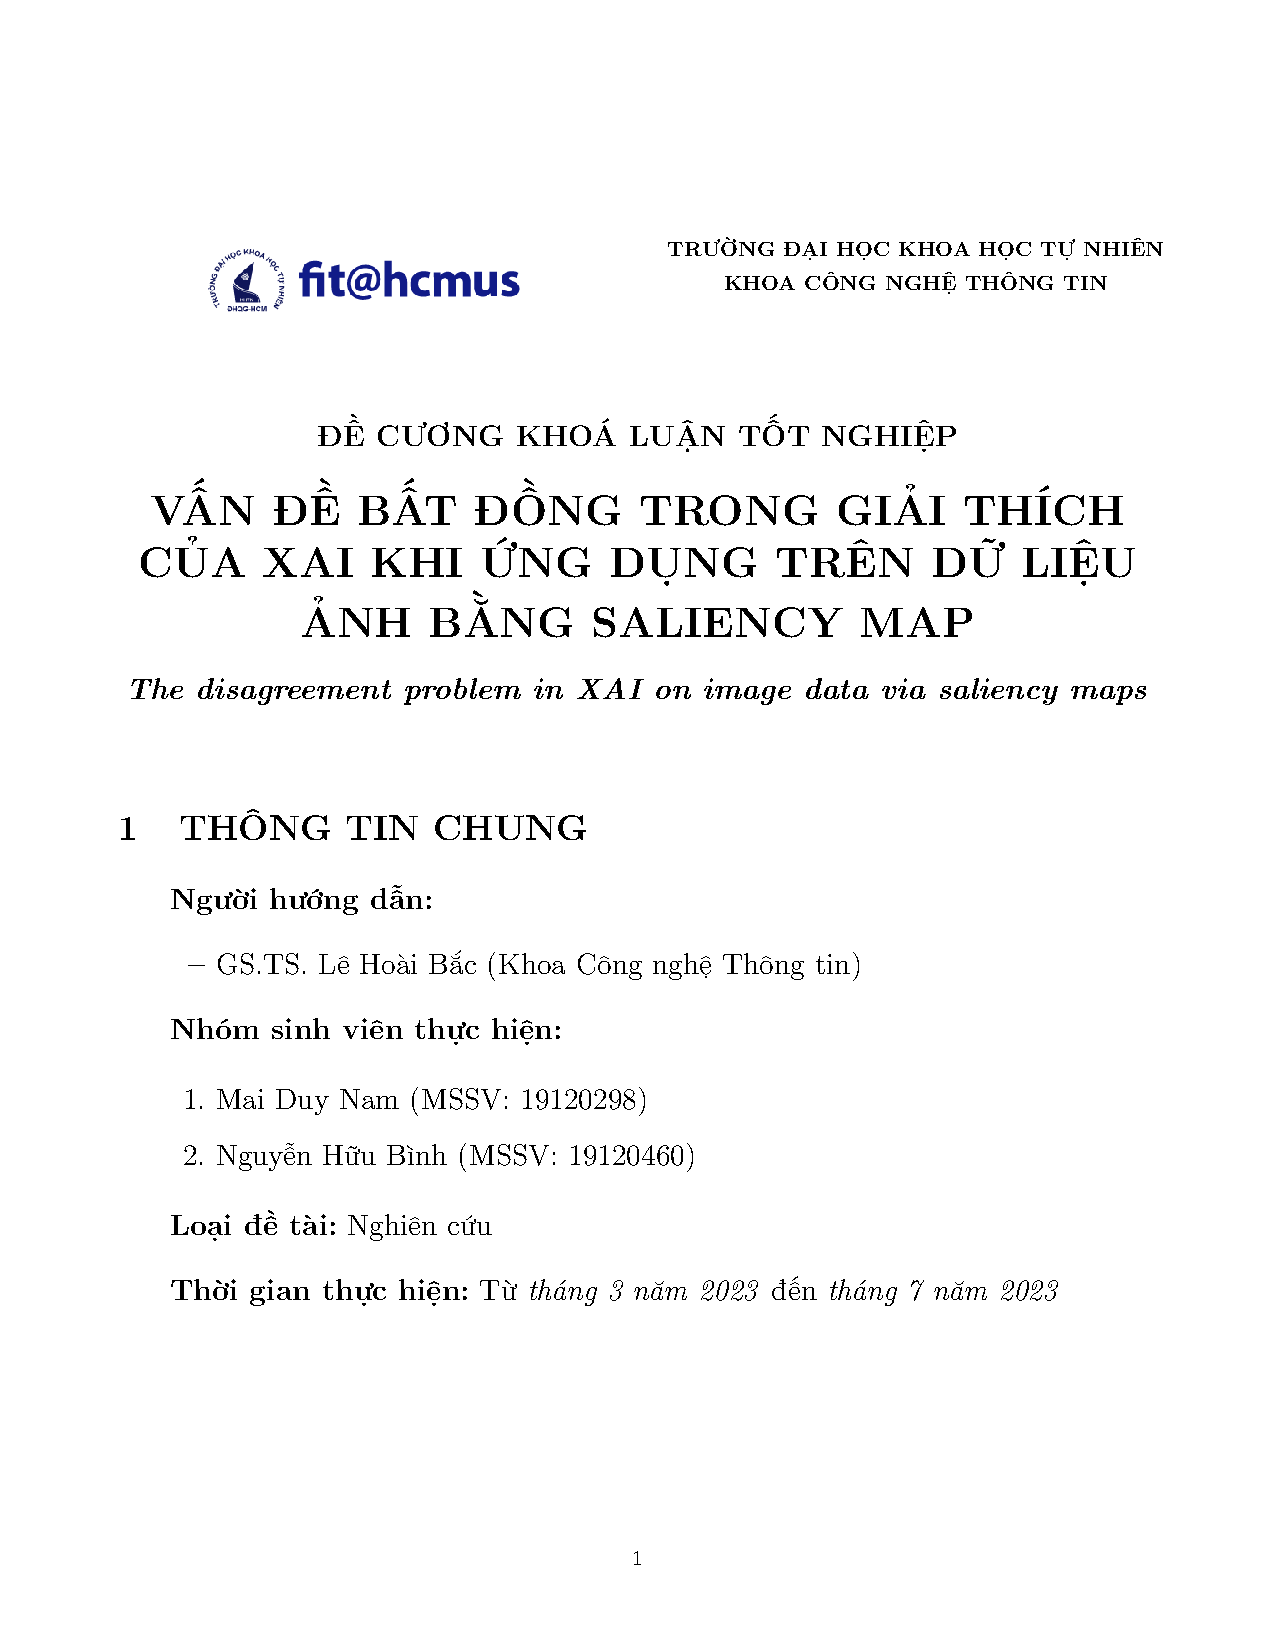
\includepdf[pages=-]{Resources/Proposal.pdf}
% Theo mẫu \href{https://www.overleaf.com/read/jwrxbcrmkgfh}{đề cương} đã điền và nộp cho giáo vụ \textit{(phải có chữ kí của giảng viên hướng dẫn)}.

% Mục lục, danh sách hình, danh sách bảng
\phantomsection
\addcontentsline{toc}{chapter}{Table of contents}
\tableofcontents
\listoffigures
\listoftables

\phantomsection
\addcontentsline{toc}{chapter}{Abstract}
\chapter*{Abstract}
\label{abstract}
Deep learning models have become increasingly complex and accurate, making them essential in various real-world applications like healthcare and security. Understanding the inner workings of these complex ``black box'' models is crucial for their appropriate use, creation, and trust. Explainable Artificial Intelligence (XAI) aims to make these complex systems interpretable through different methods, including saliency maps for convolutional neural networks. However, there is a growing concern about the ``disagreement problem,'' where explanation methods produce inconsistent and sometimes contradictory explanations. While this problem has been acknowledged for various explanation methods, disagreements within saliency methods have not been thoroughly explored. This thesis addresses this gap by measuring the extent of disagreement among popular saliency techniques using established metrics. We evaluated the disagreement for \numExperimentedMethods\ different saliency methods over two black boxes and found significant disagreement among saliency map explanations. Moreover, we observed complex patterns of disagreement, indicating that the disagreement problem depends not only on the type of explanation method but also on the specific model being explained. We also identified limitations in current measurement metrics and encourage researchers to develop new, robust metrics that can effectively capture various aspects of explanation disagreement.


\clearpage

\pagenumbering{arabic} % Đánh số 1, 2, 3, ...

% Các chương nội dung
\chapter{Conclusion}
\label{ch:conclusion}
In this chapter we conclude our thesis by providing a summary of our key findings, identify some drawbacks in our work and discuss future directions towards resolving the disagreement problem.

\section{Results}
This thesis delves into the disagreement problem in XAI in general and specifically examines the disagreement between explanation methods that utilize saliency maps, an area that has not been previously researched. Our study involved measuring the level of disagreement between \numExperimentedMethods\ saliency explanation methods over two black boxes, using four different metrics. Our findings can be summarized as follows:
\begin{itemize}
    \item We confirmed that there is a significant amount of disagreement in explanations between many saliency maps.
    \item We indicate that the level of inconsistency varies based on the type of black box employed.
    \item We also revealed that when applied to saliency maps, the sign agreement metric is roughly half of the feature agreement score, which may render it unnecessary for measuring disagreement.
\end{itemize}


\section{Limitations and Future Works}
\label{sec:futureWorks}
The disagreement problem is a novel issue that has yet to receive comprehensive research attention, resulting in a lack of diverse viewpoints and materials on the subject. However, we firmly believe that this is not a trivial issue and deserves greater attention. If not addressed adequately, the validity and transparency of XAI approaches, which are the key desired characteristics of XAI, may be seriously questioned. Our thesis is an attempt to explore a new aspect of this problem, and there is significant scope for further improvement.

We acknowledge some limitations of our work and suggest potential directions for future research. Firstly, we only tested the disagreement problem on a single dataset with one classification task. We believe that further researches on a wider range of datasets and black boxes will reveal many useful insights. Secondly, as we noted, the existing metrics are insufficient to capture the full extent of disagreement, and new metrics can be developed to address this limitation. Thirdly, while the existence of disagreement has been acknowledged, a thorough and systematic investigation into the reasons for disagreement has yet to be conducted. Future work should focus on uncovering the underlying reasons for this disagreement. Finally, we urge the XAI community to attach greater importance to this problem, as the goal of XAI is to assist humans in understanding machine learning and deep learning algorithms and to make them more interpretable, rather than introducing further confusion by providing inconsistent or contradictory explanations.

\chapter{Conclusion}
\label{ch:conclusion}
In this chapter we conclude our thesis by providing a summary of our key findings, identify some drawbacks in our work and discuss future directions towards resolving the disagreement problem.

\section{Results}
This thesis delves into the disagreement problem in XAI in general and specifically examines the disagreement between explanation methods that utilize saliency maps, an area that has not been previously researched. Our study involved measuring the level of disagreement between \numExperimentedMethods\ saliency explanation methods over two black boxes, using four different metrics. Our findings can be summarized as follows:
\begin{itemize}
    \item We confirmed that there is a significant amount of disagreement in explanations between many saliency maps.
    \item We indicate that the level of inconsistency varies based on the type of black box employed.
    \item We also revealed that when applied to saliency maps, the sign agreement metric is roughly half of the feature agreement score, which may render it unnecessary for measuring disagreement.
\end{itemize}


\section{Limitations and Future Works}
\label{sec:futureWorks}
The disagreement problem is a novel issue that has yet to receive comprehensive research attention, resulting in a lack of diverse viewpoints and materials on the subject. However, we firmly believe that this is not a trivial issue and deserves greater attention. If not addressed adequately, the validity and transparency of XAI approaches, which are the key desired characteristics of XAI, may be seriously questioned. Our thesis is an attempt to explore a new aspect of this problem, and there is significant scope for further improvement.

We acknowledge some limitations of our work and suggest potential directions for future research. Firstly, we only tested the disagreement problem on a single dataset with one classification task. We believe that further researches on a wider range of datasets and black boxes will reveal many useful insights. Secondly, as we noted, the existing metrics are insufficient to capture the full extent of disagreement, and new metrics can be developed to address this limitation. Thirdly, while the existence of disagreement has been acknowledged, a thorough and systematic investigation into the reasons for disagreement has yet to be conducted. Future work should focus on uncovering the underlying reasons for this disagreement. Finally, we urge the XAI community to attach greater importance to this problem, as the goal of XAI is to assist humans in understanding machine learning and deep learning algorithms and to make them more interpretable, rather than introducing further confusion by providing inconsistent or contradictory explanations.

\chapter{Conclusion}
\label{ch:conclusion}
In this chapter we conclude our thesis by providing a summary of our key findings, identify some drawbacks in our work and discuss future directions towards resolving the disagreement problem.

\section{Results}
This thesis delves into the disagreement problem in XAI in general and specifically examines the disagreement between explanation methods that utilize saliency maps, an area that has not been previously researched. Our study involved measuring the level of disagreement between \numExperimentedMethods\ saliency explanation methods over two black boxes, using four different metrics. Our findings can be summarized as follows:
\begin{itemize}
    \item We confirmed that there is a significant amount of disagreement in explanations between many saliency maps.
    \item We indicate that the level of inconsistency varies based on the type of black box employed.
    \item We also revealed that when applied to saliency maps, the sign agreement metric is roughly half of the feature agreement score, which may render it unnecessary for measuring disagreement.
\end{itemize}


\section{Limitations and Future Works}
\label{sec:futureWorks}
The disagreement problem is a novel issue that has yet to receive comprehensive research attention, resulting in a lack of diverse viewpoints and materials on the subject. However, we firmly believe that this is not a trivial issue and deserves greater attention. If not addressed adequately, the validity and transparency of XAI approaches, which are the key desired characteristics of XAI, may be seriously questioned. Our thesis is an attempt to explore a new aspect of this problem, and there is significant scope for further improvement.

We acknowledge some limitations of our work and suggest potential directions for future research. Firstly, we only tested the disagreement problem on a single dataset with one classification task. We believe that further researches on a wider range of datasets and black boxes will reveal many useful insights. Secondly, as we noted, the existing metrics are insufficient to capture the full extent of disagreement, and new metrics can be developed to address this limitation. Thirdly, while the existence of disagreement has been acknowledged, a thorough and systematic investigation into the reasons for disagreement has yet to be conducted. Future work should focus on uncovering the underlying reasons for this disagreement. Finally, we urge the XAI community to attach greater importance to this problem, as the goal of XAI is to assist humans in understanding machine learning and deep learning algorithms and to make them more interpretable, rather than introducing further confusion by providing inconsistent or contradictory explanations.

\chapter{Conclusion}
\label{ch:conclusion}
In this chapter we conclude our thesis by providing a summary of our key findings, identify some drawbacks in our work and discuss future directions towards resolving the disagreement problem.

\section{Results}
This thesis delves into the disagreement problem in XAI in general and specifically examines the disagreement between explanation methods that utilize saliency maps, an area that has not been previously researched. Our study involved measuring the level of disagreement between \numExperimentedMethods\ saliency explanation methods over two black boxes, using four different metrics. Our findings can be summarized as follows:
\begin{itemize}
    \item We confirmed that there is a significant amount of disagreement in explanations between many saliency maps.
    \item We indicate that the level of inconsistency varies based on the type of black box employed.
    \item We also revealed that when applied to saliency maps, the sign agreement metric is roughly half of the feature agreement score, which may render it unnecessary for measuring disagreement.
\end{itemize}


\section{Limitations and Future Works}
\label{sec:futureWorks}
The disagreement problem is a novel issue that has yet to receive comprehensive research attention, resulting in a lack of diverse viewpoints and materials on the subject. However, we firmly believe that this is not a trivial issue and deserves greater attention. If not addressed adequately, the validity and transparency of XAI approaches, which are the key desired characteristics of XAI, may be seriously questioned. Our thesis is an attempt to explore a new aspect of this problem, and there is significant scope for further improvement.

We acknowledge some limitations of our work and suggest potential directions for future research. Firstly, we only tested the disagreement problem on a single dataset with one classification task. We believe that further researches on a wider range of datasets and black boxes will reveal many useful insights. Secondly, as we noted, the existing metrics are insufficient to capture the full extent of disagreement, and new metrics can be developed to address this limitation. Thirdly, while the existence of disagreement has been acknowledged, a thorough and systematic investigation into the reasons for disagreement has yet to be conducted. Future work should focus on uncovering the underlying reasons for this disagreement. Finally, we urge the XAI community to attach greater importance to this problem, as the goal of XAI is to assist humans in understanding machine learning and deep learning algorithms and to make them more interpretable, rather than introducing further confusion by providing inconsistent or contradictory explanations.

\chapter{Conclusion}
\label{ch:conclusion}
In this chapter we conclude our thesis by providing a summary of our key findings, identify some drawbacks in our work and discuss future directions towards resolving the disagreement problem.

\section{Results}
This thesis delves into the disagreement problem in XAI in general and specifically examines the disagreement between explanation methods that utilize saliency maps, an area that has not been previously researched. Our study involved measuring the level of disagreement between \numExperimentedMethods\ saliency explanation methods over two black boxes, using four different metrics. Our findings can be summarized as follows:
\begin{itemize}
    \item We confirmed that there is a significant amount of disagreement in explanations between many saliency maps.
    \item We indicate that the level of inconsistency varies based on the type of black box employed.
    \item We also revealed that when applied to saliency maps, the sign agreement metric is roughly half of the feature agreement score, which may render it unnecessary for measuring disagreement.
\end{itemize}


\section{Limitations and Future Works}
\label{sec:futureWorks}
The disagreement problem is a novel issue that has yet to receive comprehensive research attention, resulting in a lack of diverse viewpoints and materials on the subject. However, we firmly believe that this is not a trivial issue and deserves greater attention. If not addressed adequately, the validity and transparency of XAI approaches, which are the key desired characteristics of XAI, may be seriously questioned. Our thesis is an attempt to explore a new aspect of this problem, and there is significant scope for further improvement.

We acknowledge some limitations of our work and suggest potential directions for future research. Firstly, we only tested the disagreement problem on a single dataset with one classification task. We believe that further researches on a wider range of datasets and black boxes will reveal many useful insights. Secondly, as we noted, the existing metrics are insufficient to capture the full extent of disagreement, and new metrics can be developed to address this limitation. Thirdly, while the existence of disagreement has been acknowledged, a thorough and systematic investigation into the reasons for disagreement has yet to be conducted. Future work should focus on uncovering the underlying reasons for this disagreement. Finally, we urge the XAI community to attach greater importance to this problem, as the goal of XAI is to assist humans in understanding machine learning and deep learning algorithms and to make them more interpretable, rather than introducing further confusion by providing inconsistent or contradictory explanations.

\chapter{Conclusion}
\label{ch:conclusion}
In this chapter we conclude our thesis by providing a summary of our key findings, identify some drawbacks in our work and discuss future directions towards resolving the disagreement problem.

\section{Results}
This thesis delves into the disagreement problem in XAI in general and specifically examines the disagreement between explanation methods that utilize saliency maps, an area that has not been previously researched. Our study involved measuring the level of disagreement between \numExperimentedMethods\ saliency explanation methods over two black boxes, using four different metrics. Our findings can be summarized as follows:
\begin{itemize}
    \item We confirmed that there is a significant amount of disagreement in explanations between many saliency maps.
    \item We indicate that the level of inconsistency varies based on the type of black box employed.
    \item We also revealed that when applied to saliency maps, the sign agreement metric is roughly half of the feature agreement score, which may render it unnecessary for measuring disagreement.
\end{itemize}


\section{Limitations and Future Works}
\label{sec:futureWorks}
The disagreement problem is a novel issue that has yet to receive comprehensive research attention, resulting in a lack of diverse viewpoints and materials on the subject. However, we firmly believe that this is not a trivial issue and deserves greater attention. If not addressed adequately, the validity and transparency of XAI approaches, which are the key desired characteristics of XAI, may be seriously questioned. Our thesis is an attempt to explore a new aspect of this problem, and there is significant scope for further improvement.

We acknowledge some limitations of our work and suggest potential directions for future research. Firstly, we only tested the disagreement problem on a single dataset with one classification task. We believe that further researches on a wider range of datasets and black boxes will reveal many useful insights. Secondly, as we noted, the existing metrics are insufficient to capture the full extent of disagreement, and new metrics can be developed to address this limitation. Thirdly, while the existence of disagreement has been acknowledged, a thorough and systematic investigation into the reasons for disagreement has yet to be conducted. Future work should focus on uncovering the underlying reasons for this disagreement. Finally, we urge the XAI community to attach greater importance to this problem, as the goal of XAI is to assist humans in understanding machine learning and deep learning algorithms and to make them more interpretable, rather than introducing further confusion by providing inconsistent or contradictory explanations.


% Công trình của tác giả (nếu không có thì comment 02 dòng dưới)
% \addcontentsline{toc}{chapter}{Danh mục công trình của tác giả}
% \chapter*{Danh mục công trình của tác giả}
% \label{Appendix1}

\begin{enumerate}
\item Tạp chí ABC
\item Tạp chí XYZ
\end{enumerate}

% In tài liệu tham khảo
\addcontentsline{toc}{chapter}{References}
\printbibheading[title={References}]

% \printbibliography[heading=subbibliography, title={Tiếng Việt}, keyword=Viet, resetnumbers=true]

\DeclareNameAlias{sortname}{family-given}
\DeclareNameAlias{default}{family-given}

\printbibliography[heading=subbibliography, title={Tiếng Anh}]

%, notkeyword=Viet]
%, resetnumbers=4] 
% ===================================================================== %
% CHÚ Ý: phải gán lại resetnumbers=số tài liệu tham khảo tiếng Việt + 1 %
% ===================================================================== %

% Phần phụ lục
% \appendix

\chapter{Ngữ pháp tiếng Việt}
\label{Appendix1}

Đây là phụ lục.
% \chapter{Ngữ pháp tiếng Nôm}
\label{Appendix2}

Đây là phụ lục 2.

\end{document} 